\section{Task 2: FRECA, Compliance Auditing with Grounded LLM Reasoning}
\label{sec:task2}

\subsection{Problem and Data}
\label{sec:t2-problem}

Given nine heterogeneous evidence files per farm export establishment (Registered
Establishment, RE), the system must audit compliance against 41 checking points (CPs)
drawn from the \emph{Export Control (Plants and Plant Products) Rules 2021}, emitting
\texttt{1} (compliant), \texttt{0} (non-compliant) or \texttt{N/A} per CP. Three hard
constraints govern the design: no hard-coded compliance logic anywhere in the pipeline,
LLM-API-only reasoning, and reproducibility.

The corpus has 99 raw folders that resolve to 100 logical cases, each with 7
\texttt{.docx} and 2 \texttt{.xlsx} tracks, and a 132-page policy document with 184
sections (Table~\ref{tab:t2-dataset} in Appendix~\ref{app:t2}). No labels were
provided; we hand-labelled a 10-case development set for internal measurement only,
and its labels were not independently verified. A median case is about 8.2K words
(22--26K tokens), so a whole case fits in one context window. Exploratory analysis
(Exp.~B1) found that one folder holds two complete establishments under the same RE
number (the ``missing'' 100th case), two folders lack the registration form, and some
apparent signals are generation noise.

\subsection{Submitted System}
\label{sec:t2-arch}

\begin{figure}[t]
\centering
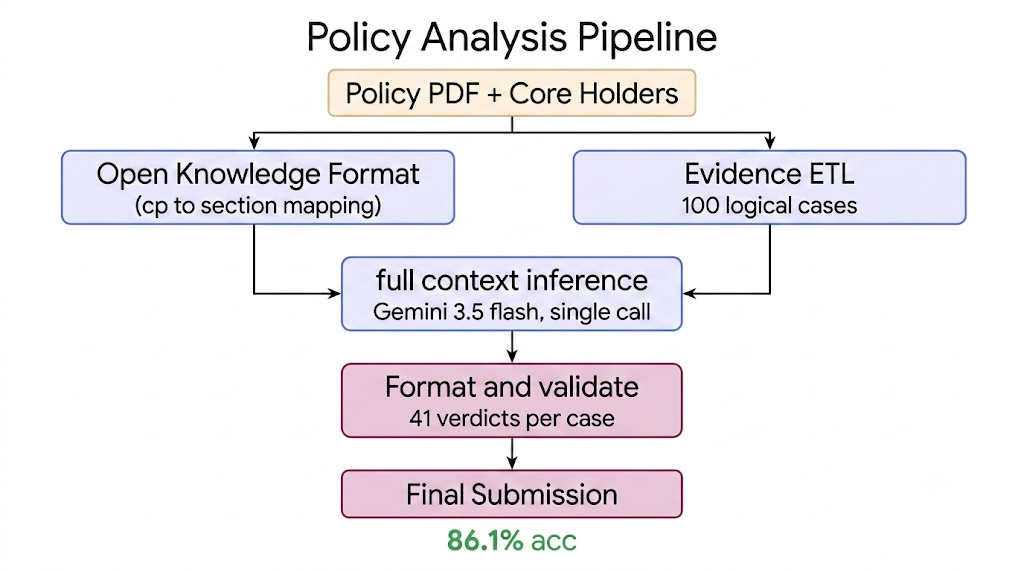
\includegraphics[width=0.52\textwidth]{task2_architecture.png}
\caption{Task~2 pipeline: an offline Open Knowledge Format (CP-to-section grounding)
and a per-case deterministic evidence ETL feed a single full-context call to
Gemini~3.5~Flash, followed by formatting and validation into the submission matrix.}
\label{fig:t2-arch}
\end{figure}

The pipeline (Fig.~\ref{fig:t2-arch}) has four phases.


\noindent\textbf{Phase 1: Open Knowledge Format (OKF), offline, once.} The policy PDF is chunked
into 184 sections by a deterministic regex on section headers. A one-time LLM pass
reads the statute text and maps each of the 41 CPs to its governing section(s),
producing a YAML-cited bundle of 18 unique sections (deduplicated from 64 citation
instances). It is stored with the system and can be re-derived on demand.

\noindent\textbf{Phase 2: deterministic evidence ETL, per case.} A canonical logical-case manifest
resolves the 99 folders into 100 cases by splitting the doubled folder;
an ingestion step flattens \texttt{.docx}/\texttt{.xlsx} files into track-tagged
markdown, preserving table structure, tolerating missing tracks and sorting
lexicographically for reproducibility. This layer contains no compliance logic.

\noindent\textbf{Phase 3: full-context inference, per case.} One prompt per case
($\sim$44K tokens) holds the complete evidence, the OKF bundle (CP texts and governing
sections) and a persona prompt enforcing identity anchoring, boilerplate-versus-signal
discipline and \texttt{N/A} discipline. Model: Gemini~3.5~Flash~\cite{geminiteam2023},
temperature 0, reasoning enabled; temperature~0 does not guarantee identical outputs
across runs. Output: structured JSON with 41 verdicts, reasoning and confidence.
% TODO: give the exact model string / snapshot ID used for the 100-case run

\noindent\textbf{Phase 4: formatting and validation.} Verdicts are enum-validated into the
submission matrix (RE Number~+~CP1\ldots CP41).

The ETL performs pure extraction and the CP-to-section mapping is LLM-derived from the
statute, so neither contains compliance rules. The persona prompt, however, carries a
CP38-motivated instruction added after Exp.~B9. We distinguish encoding a checking
point's \emph{requirement} (what the governing text obliges) from hard-coding the
\emph{expected answer} (instructing which verdict to emit for a specific evidence
string); the former is legitimate grounding, the latter is non-compliant. The added
wording is general in form --- ``where a register row has both a fixed target and a
case-specific status/verification note, the status note is the signal, not the
target'' --- but its examples name the concrete strings ``2-year retention verified''
and ``migration in progress'' / ``pending'' that separate compliant from
non-compliant rows in this dataset. It is therefore a general interpretation rule
with CP38-answer-specific examples, so the no-hard-coding constraint holds only
partially. The intervention was developed and scored on the same ten dev cases and
was never evaluated on unseen cases, so we do not claim the constraint is fully
satisfied.

\noindent\textbf{Production run} (Exp.~B14). With a 240-second per-call timeout and
per-case checkpointing, all 100 cases completed with no blanks and no parse failures,
using 4{,}493{,}869 tokens ($\sim$44.9K per case); the run was resumed four times after
key changes and credit or rate-limit stops without losing progress. The output holds
3{,}118 \texttt{1}, 982 \texttt{0} (23.95\%, against 17.6\% in the dev gold) and no
\texttt{N/A}. The 100th case, the second establishment in the doubled folder, was submitted under a
provisional ID.

\subsection{Development Path}
\label{sec:t2-experiments}


\noindent\textbf{Model choice.} With identical prompts, grounding and evidence
(Exp.~B4; Table~\ref{tab:t2-bakeoff} in Appendix~\ref{app:t2}), Gemini~3.5~Flash
reached 86.1\% against 76.6\% for Nemotron Ultra and 81.5\% for DeepSeek~V4~Pro.
Sonnet~5 scored highest (91.0\%) but was withdrawn
because the submission had to be reproducible through the team's own API key (an
access constraint, not a quality judgement); Gemini~3.5~Flash was the best model that
met it.

\noindent\textbf{Full context beat retrieval.} A hybrid RAG
branch~\cite{lewis2020rag} (BM25~\cite{robertson2009bm25} and bge-small dense
retrieval~\cite{xiao2024bge}, weighted fusion, ColBERT~\cite{khattab2020colbert}
rerank) scored 74.9\% at 610K tokens against 86.1\% at 442K for full context
(Exp.~B6). When a case fits in one
context window, retrieval only adds the risk of missing a decisive sentence: the
``maintained in Mandarin'' sentence was retrieved only $\sim$56\% of the time.

\noindent\textbf{Fewer calls.} The call architecture went from per-element,
per-persona calls (13 per case, megabyte-scale prompts) to a 3-persona ensemble
(3 calls, $\sim$215K tokens, with a hard-coded majority threshold) to the single
full-context call ($\sim$44K tokens) (Exp.~B8). On one case a Haiku persona ensemble
scored 70.7\% against 92.7\% for a single Sonnet pass at lower token cost (Exp.~B5);
this confounds model tier with ensembling, and we did not test a strong-model ensemble.

\noindent\textbf{Boilerplate versus signal.} CP38 (record retention) was being decided
from a date-range string that is byte-identical across compliant and non-compliant
cases. Telling the model that the per-case status note is the signal took CP38 from
4/10 to 10/10 on the in-sample dev set. This was measured on the Sonnet~5 development
run, \emph{not} on the submitted Gemini~3.5~Flash model, so it is a prompt-development
observation rather than a result of the submitted system; the same class of fix is
still needed for CP37 (Exp.~B10).

\noindent\textbf{Error analysis} on the dev set (Exps.~B10--B13): the model never emits
\texttt{N/A} (all 8 gold-\texttt{N/A} cells were predicted \texttt{1}), Element-4
(traceability) is weakest at 77.7\%, and CP39's gold is internally inconsistent.

\subsection{Results}
\label{sec:t2-results}

The organisers scored the submission at accuracy 0.7818, precision 0.7758, recall
0.7818 and F$_\beta$ 0.7783. Recall equal to accuracy indicates support-weighted
averaging. The 0.861 figure is \emph{in-sample development accuracy} on a 10-case
set that we self-labelled and then used to tune the prompts (including the CP38
wording); it is not an estimate of generalization, and we do not report it as such.
The official accuracy is 7.9 points below that in-sample number and below the worst
dev case (dev cases range from 80.5\% to 95.1\%; Exp.~B11), so the gap is not sampling
noise within the dev set. However, because no independent labelled evaluation set
exists, the cause of the official-score gap \emph{cannot be established from the
available evidence}; the following are hypotheses only: the dev labels are
self-assigned and unverified; the CP38 prompt was tuned on the dev set; CP39's gold
is inconsistent; and $n=10$. Over-flagging is a further hypothesis, since the
production run predicts \texttt{0} more often than the dev gold and class-0 precision
on the dev set was only 0.616.

\noindent\textbf{Limitations.} The ten dev cases are self-labelled and were used to
tune prompts, so dev accuracy is not held-out accuracy; the CP37--39 analysis used the
Sonnet run rather than the submitted model; the OKF was not ablated, and only 12 of 41
CPs were mapped identically by two mapping models; ensembling was not tested with a
strong base model; and the exact model snapshot is not recorded
(Appendix~\ref{sec:t2-limits}).
